\documentclass[12pt]{article}
%\documentclass{article}

\usepackage{times}
\usepackage[final]{graphicx}
\usepackage{hyperref}

\setlength{\topmargin}{-0.5in}
\setlength{\oddsidemargin}{0in}
\setlength{\evensidemargin}{0in}
\setlength{\textwidth}{6.5in}
\setlength{\textheight}{9.0in}

\begin{document}

\centerline{\bf \Large CS295/CS395/CSYS395: \href{CS295_395_Syllabus.pdf}{\underline{Evolutionary Robotics}}}

\vspace{0.5cm}

\centerline{\bf \large Programming Assignment 6 of 10}

\vspace{0.5cm}

\centerline{\large Assigned: Friday, October 7, 2011}

\vspace{0.5cm}

\centerline{\large Due: Friday, October 14, 2011 by midnight}

\vspace{0.5cm}

\noindent \textbf{Description:} In this week's assignment you will be adding eight joints to connect together the nine body parts comprising the robot (Fig. \ref{Fig1}). You will accomplish this in the same way as for adding bodies to ODE: add one joint, compile and run the application so that you can see the effect of the addition on the simulation, only then add a second joint, and so on.

\begin{enumerate}

\item Back up Assignment\_5 on a flash drive or another computer so that you can always return to your completed fifth assignment.

\item Copy directory Assignment\_5, which contains your submitted document and the entire ODE folder. Rename the new directory Assignment\_6.

\item At the top of the test\_buggy code, add a new data structure that will store the eight joints to be created: \\
\texttt{static dJointID joints[8];}\\

\item Now create a function \texttt{CreateHinge(int index,...)} that will create a joint. You will need to pass this function a number of parameters: you need to tell it which two bodies to attach together; where the joint's fulcrum should be; and the axis of the joint. If you are unfamiliar with these concepts, refer to the Lecture 6 on physical simulation.

\item Inside this function you will use these parameters to: \\
join two bodies together (\texttt{dJointAttach(...)}), \\
set the position of the joint's fulcrum (\texttt{dJointSetHingeAnchor(...)}), and \\
set the joint's orientation (\texttt{dJointSetHingeAxis(...)}). \\
For more information about these three functions refer to ODE's documentation.

\item Create another function \texttt{DestroyHinge(int index)} that removes the joint from the simulation.

\item Add a line \texttt{CreateHinge(0,...);} that creates the first joint, which attaches the right lower leg to the right upper leg (Fig. \ref{Fig1}a). This line should be placed just after all of the bodies have been created, but before simLoop is called.

\item Add a second line \texttt{DestroyHinge(0);} after simLoop returns.

\item Compile and run the simulation in paused mode. Press CTRL-O repeatedly to step through the simulation. You should see that, as the right upper leg falls, it is stays connected to the right lower leg at the `knee'. You should see something like that of Fig. \ref{Fig1}a. Screen capture this image and store it in your document.

\item Now add the second joint that connects the left upper leg to the left lower leg, recompile and rerun.

\item Add the third joint that connects the front (into the screen) upper leg to the front lower leg, recompile and rerun.

\item Add the fourth joint that connects the back (toward the viewer) upper leg to the back lower leg, recompile and rerun. This should now produces an image like that in Fig. \ref{Fig1}b. Screen capture and store in your document.

\item Using the same procedure, add the fifth joint that connects the right upper leg to the main body. Recompile, rerun and step through the simulation to get an image like that in Fig. \ref{Fig1}c. Screen capture and copy into your document.

\item Now iteratively add the sixth, seventh and eighth joint connect the remaining three legs to the main body. The robot should now `sit down', and its legs should flatten out, producing an image as in Fig. \ref{Fig1}d.

\item We now need to constrain the range of motion of each joint. For simplicity, we will set each joint to only rotate through $[-45^o,45^o]$. To do this, you will need to add two more lines to \texttt{CreateHinge(...)}: \\
    \texttt{dJointSetHingeParam(joints[index],dParamLoStop,-45*(3.14159/180));} \\
    \texttt{dJointSetHingeParam(joints[index],dParamHiStop,+45*(3.14159/180));} \\
    What is the \texttt{x*(3.14159/180)} for?

\item Now when you recompile and rerun the simulation you should obtain an image as in Fig. \ref{Fig1}e. Screen capture and copy into your document, and submit your document.

\end{enumerate}

\begin{figure}[!t]
\centerline{
a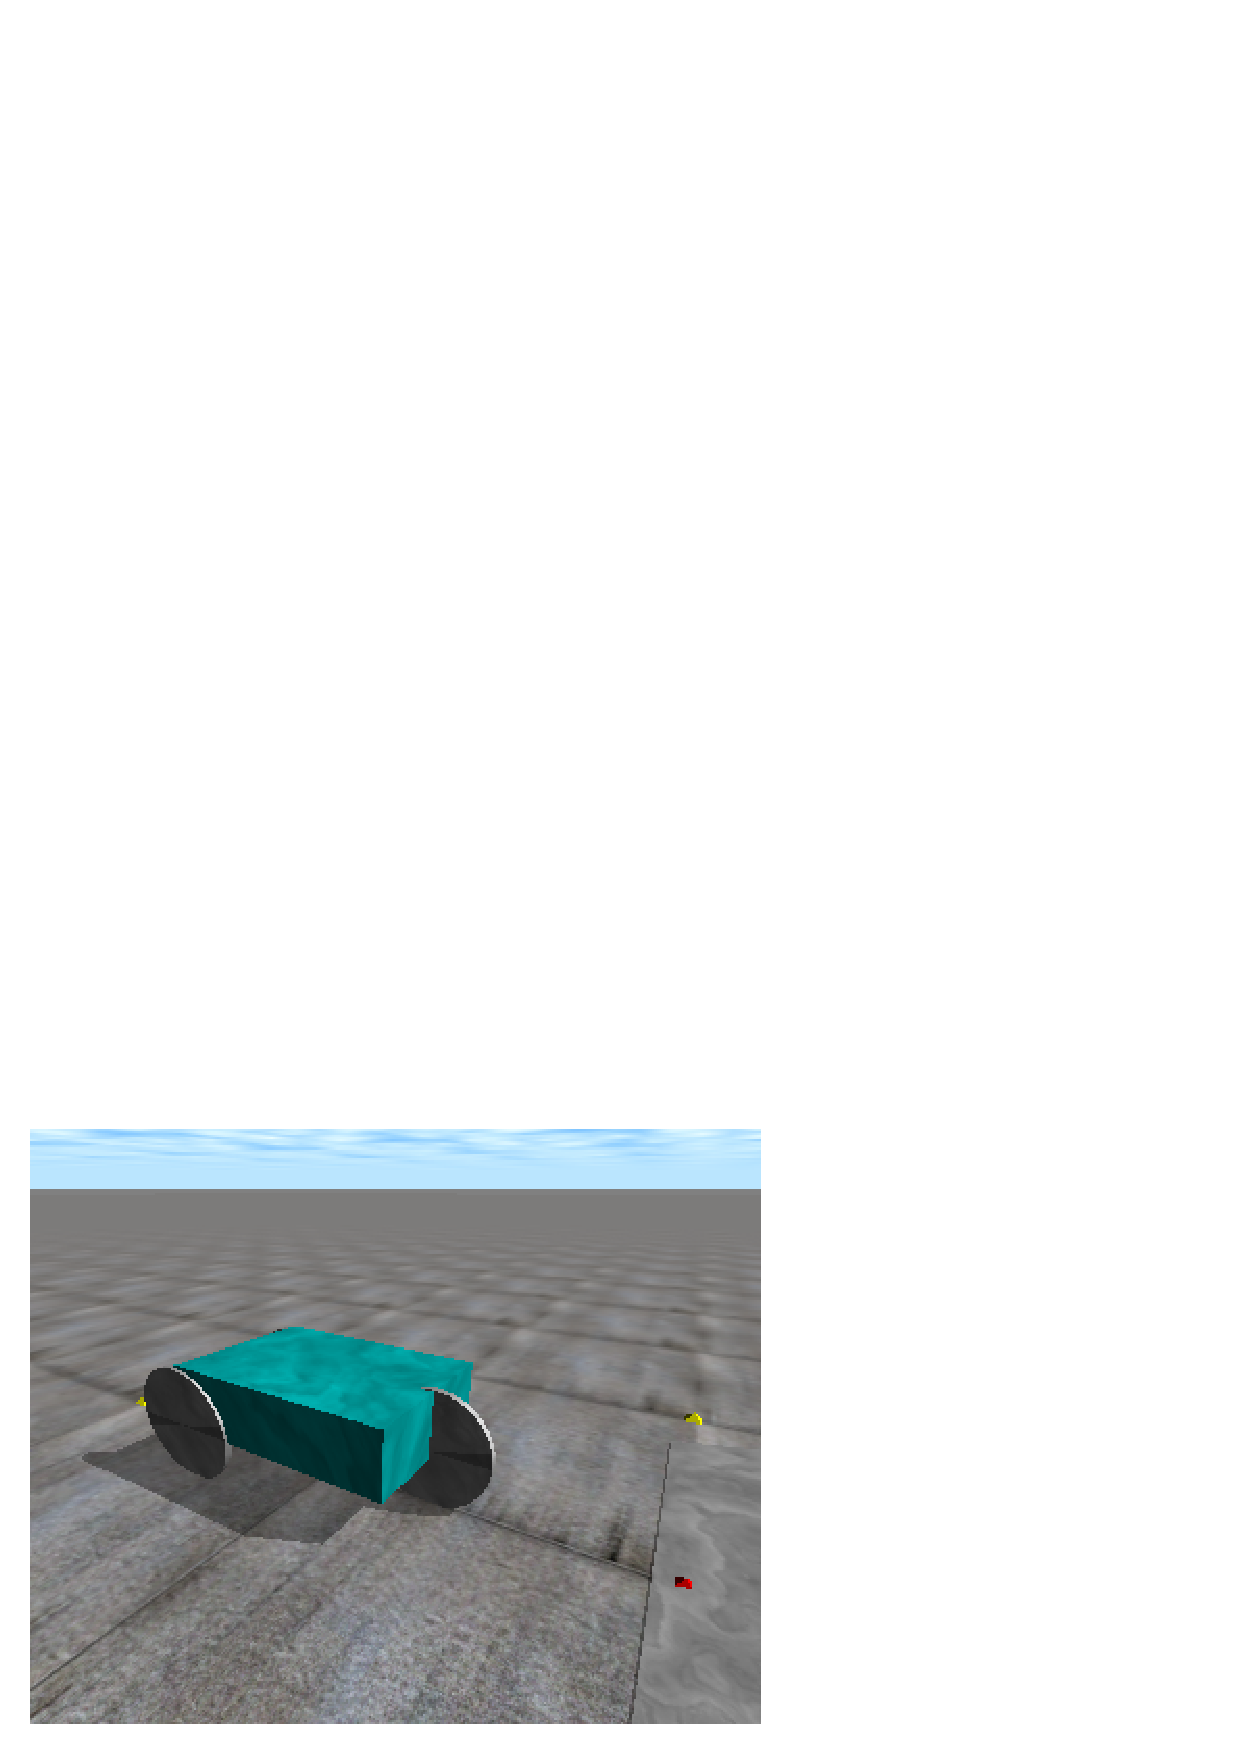
\includegraphics[width=0.25\textwidth]{Fig1a.pdf}
b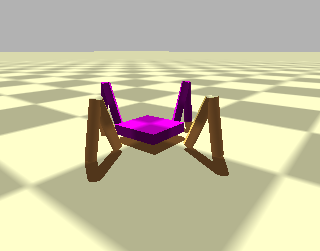
\includegraphics[width=0.25\textwidth]{Fig1b.pdf}
c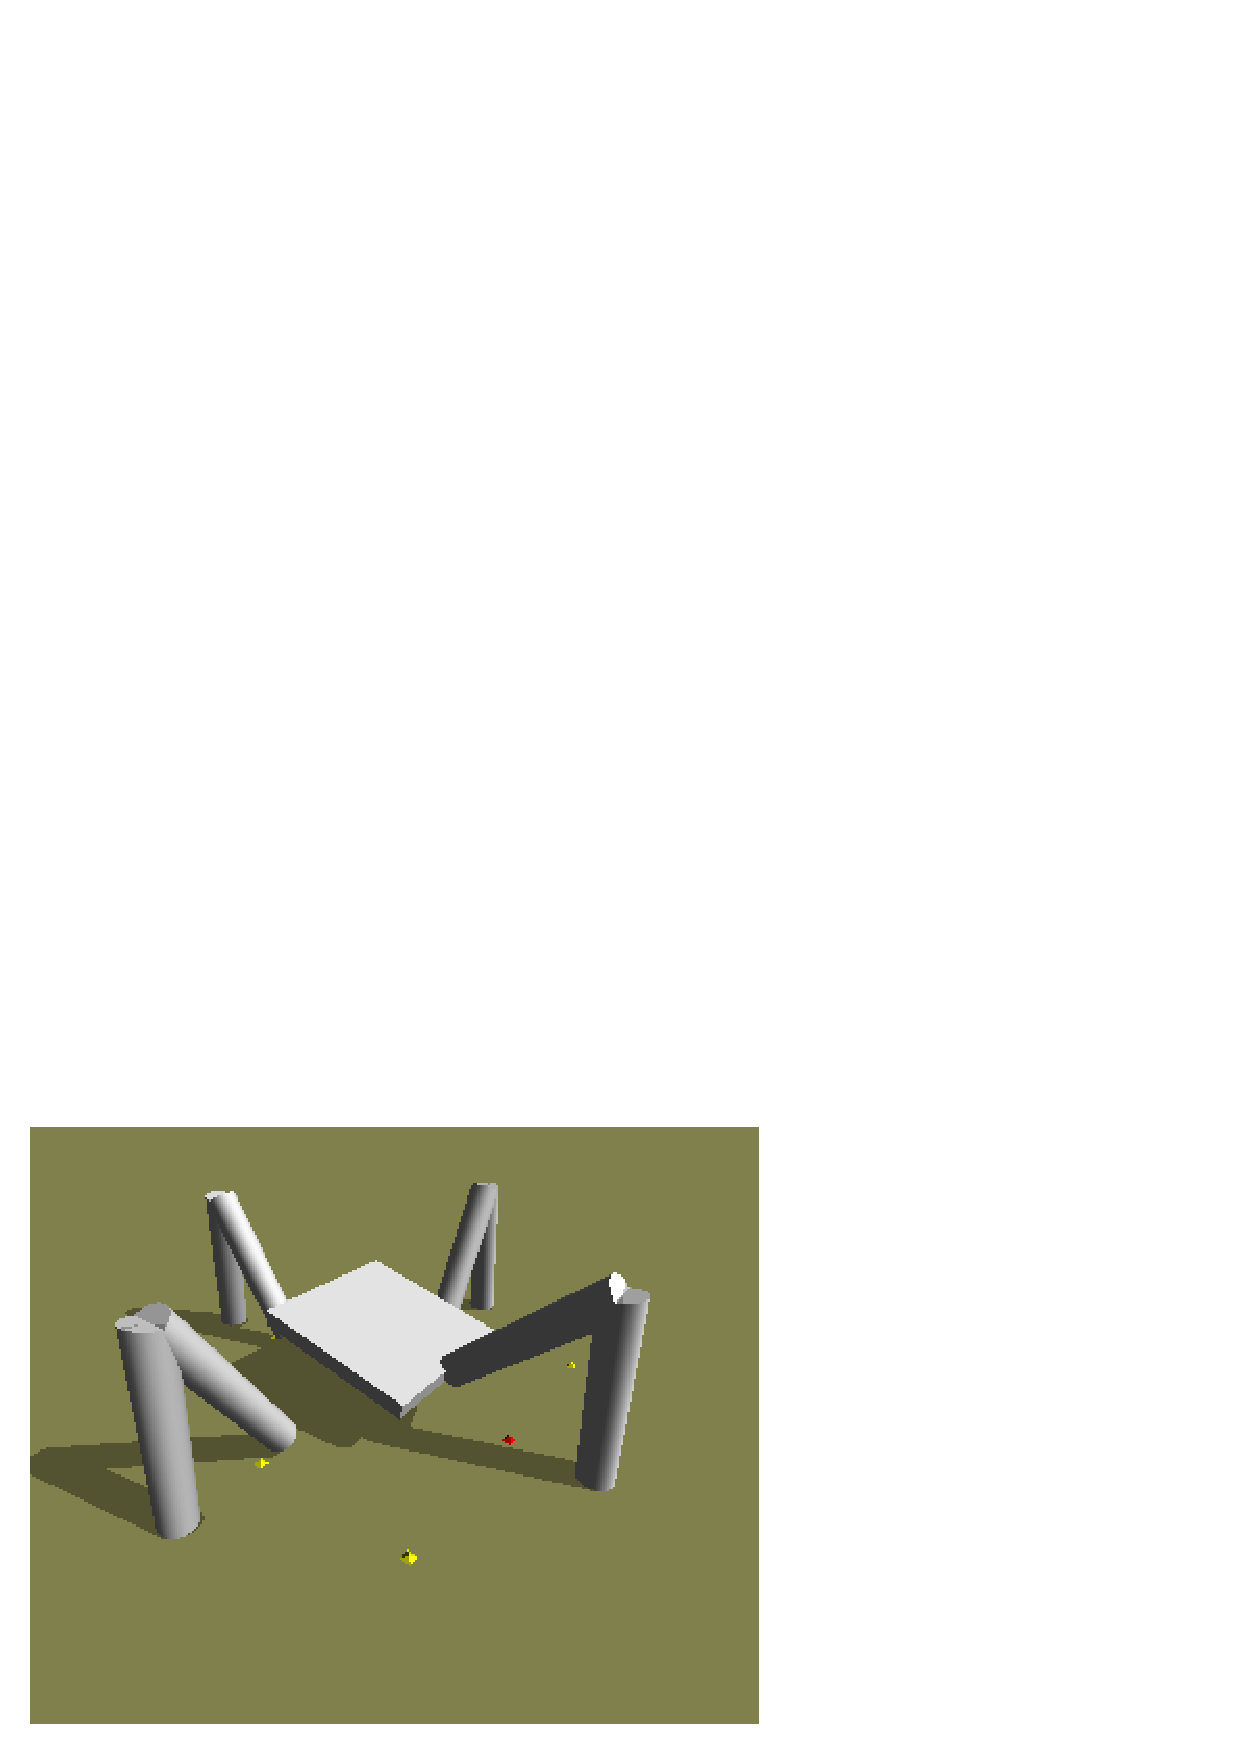
\includegraphics[width=0.25\textwidth]{Fig1c.pdf}}
\centerline{
d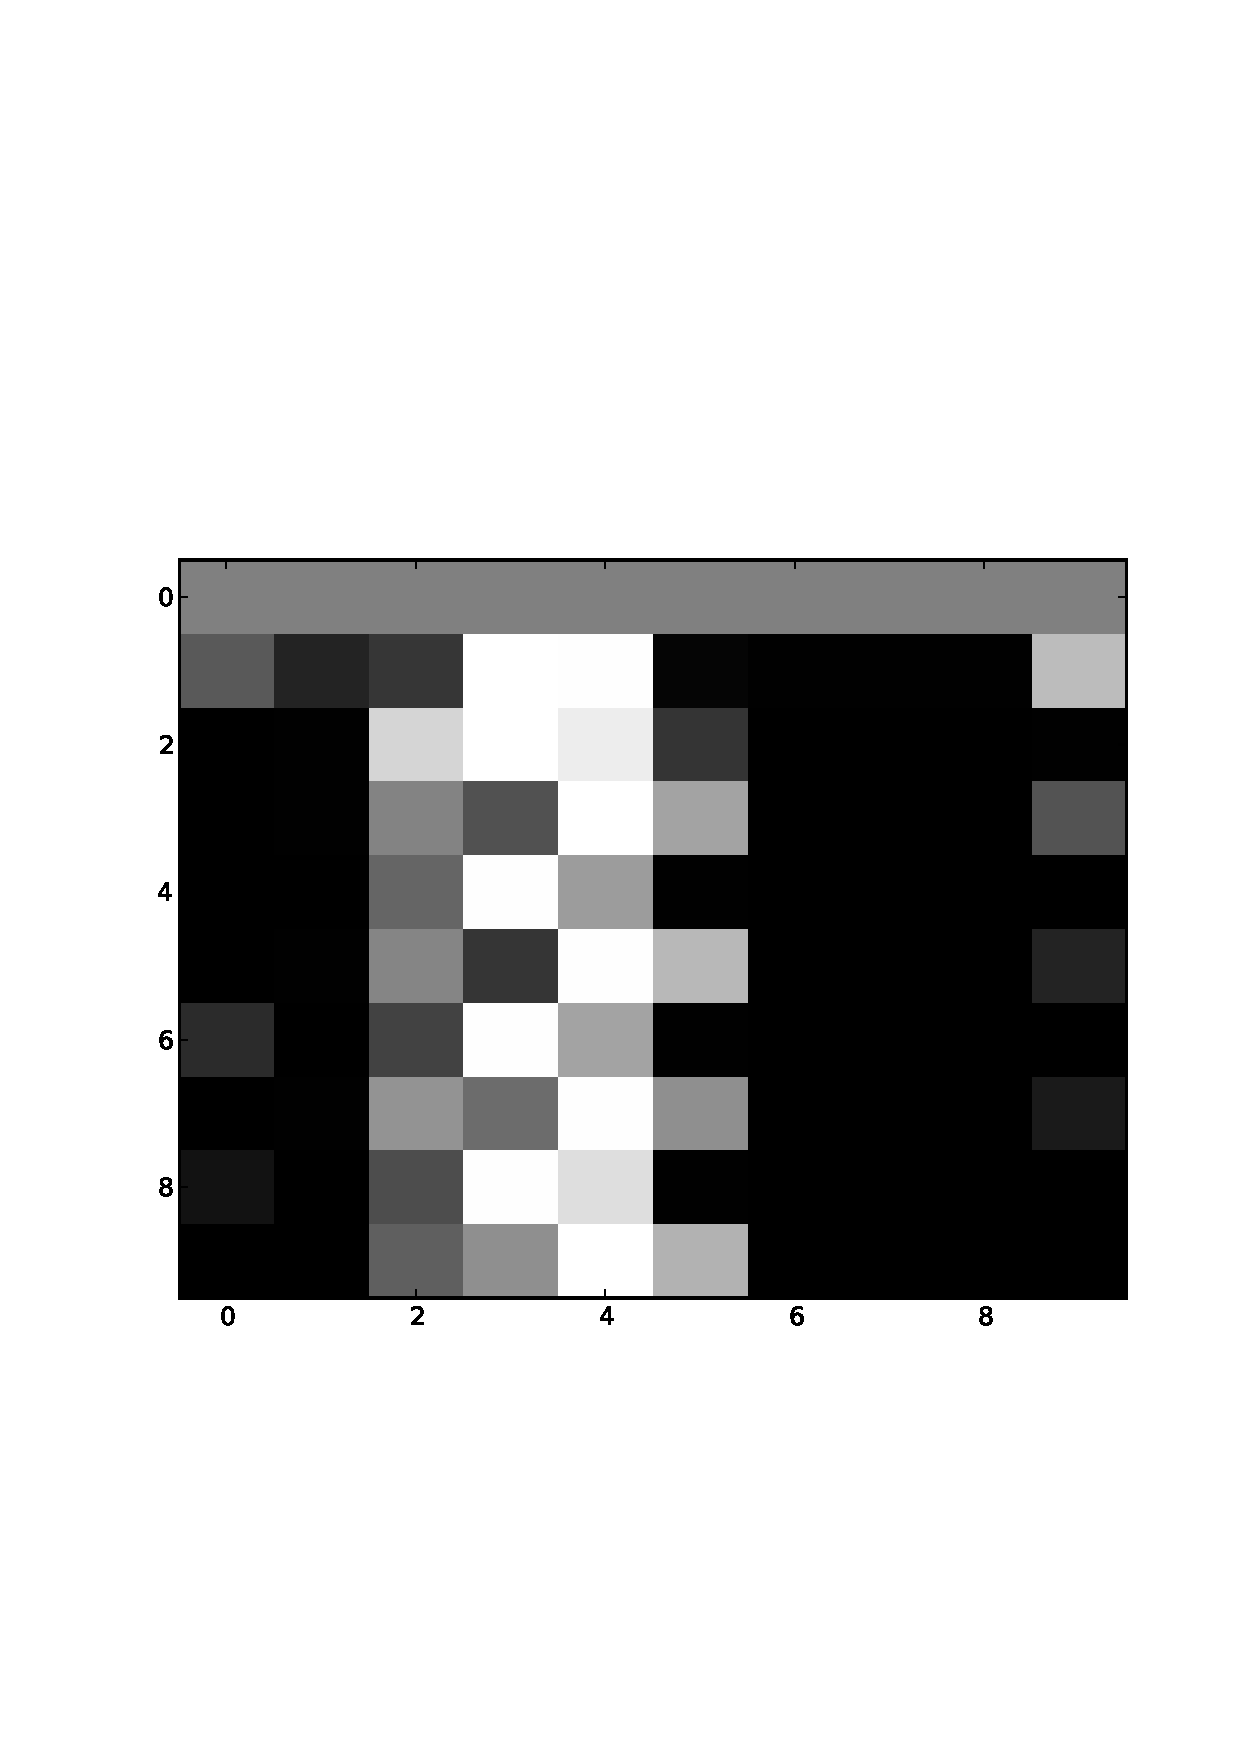
\includegraphics[width=0.25\textwidth]{Fig1d.pdf}
e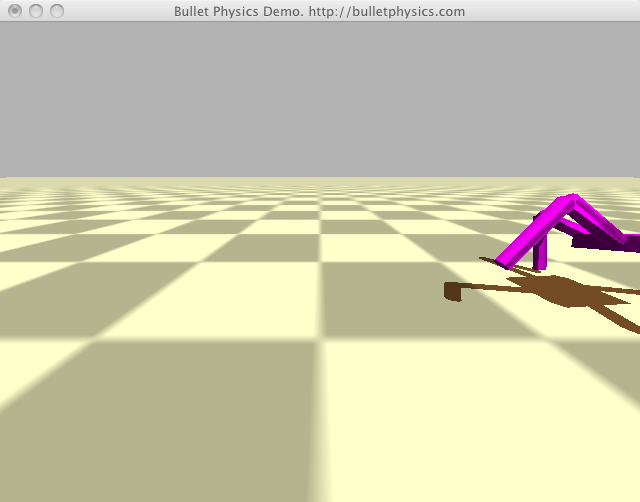
\includegraphics[width=0.25\textwidth]{Fig1e.pdf}}
\caption{Incremental addition of joints to the quadrupedal robot.}
\label{Fig1}
\end{figure}

\end{document} 
